\chapter[Automatic image generation] {Automatic image generation}
\label{cap:AIG}
\begin{Resumen}
AIG defines the ability to display any kind of graphical representation (e.g. images, pointers, schemes, etc.), based on data from any origin possible autonomously and faithfully.
\end{Resumen}
\PartialToc
\bigskip
\lettrine[lines=2]{\textbf{A}}{}utomatization of any element requires a complete and scrupulex knowledge of the original data, plus of the treatment undertaken with them. Therefore, its achievement has implied a long period of \nameref{sec:approach:software:FME} and \nameref{sec:approach:software:ArcGIS} traineeship, apart from a theoretical contents (\nameref{subsub:AIG:SLV:graph_theory}, \nameref{subsub:AIG:SLV:Voronoi} and \nameref{subsub:AIG:SLV:MDS} among others) projection towards its completion. Through a first vertebrance of the CIM file structure in FME, followed by a post-treatment image optimization performed in ArcGIS, the autor has ended up with an automatic, intelligent but still versatile and intelligent displaying process of the network layout entirely automatic. 

The openness towards performance optimizing processes altogether with the explosion of Big Data makes automatic image generation to be the order of the day in numerous engineering FoSs \cite{Software_diagrams, Deep_learning_image_to_text}. Notwithstanding, when we extrapolate this to the corporate network layout of the big electrics most of this reports are strictly confidential and merely code-oriented \cite{standard-based-SLD-AG,}. This fact forces to a severe abstraction exercise to take place, seeking to adapt the state of art actual innovations to our case of study. 

At the moment, we are deeply surrounded by intelligent AIG devices, able to mutate in function of a certain parametrization: DAR EJEMPLOS DE AIG. This unperennity recognition process is called as \nameref{subsub:AIG:SLV:graph_theory:meta_algorithms}, a variable evolution of \nameref{sub:AIG:machine_learning} ethics, giving borth to the term Automatic Machine Learning (AML). 

At the moment, multiple softwares (\hyperlink{https://github.com/iTransformers/netTransformer}{netTransformer}, \hyperlink{https://github.com/OpenNMS/opennms}{OpenNMS}, \hyperlink{https://www.docusnap.com}{Docusnap}\footnote{This licence-restricted software is also XML-based, so is our methodology.} or \hyperlink{https://www.netbraintech.com}{netBrain} among others) have been developed to easy the representation of all topologies of network diagrams. However, they remain power-limited and with a low level of automatization in regards to the requirements of Herge.


\section{Introduction}

Automatic electrical network layout generation is introduced in this work. In general, the proposed \nameref{sec:AIG:methodology} has potential in functional software testing and industrialization. The present study was pursued on the basis of the actual widget, with an aim on its automatizing, but still making use of the same corporate methods, software and principles.

Several steps were taken to progressively attack the challenge in the most rigorous manner:
\begin{description}
    
    \item - A \textbf{skill ramp-up} let the author technically identify the different elements of the electrical network in the field, and the way they were represented following corporate conventions \cite{doctrine_cod_sites, doctrine_cod_liaisons, doctrine_cod_postes}.
    
    \item - Thereupon, \textbf{taking conscience of \nameref{sec:approach:software:FME} potential}, while impregnating of its working methodology was the roughest step. Different case studies were performed to project mental skills on problem solving through this software, which progressively increased in difficulty.
    
    \item - Once FME-capable of exploiting the problem, a \textbf{familiarization with the databases}, their alphanumeric argument coding system and the way they were structured was carried out. This databases were enriched subsequently for easing meetings' agreements to achieve the bijectivity between them and the different elements representation.
    
    \item - The network skeleton once completely displayed, \textbf{image optimization processes} could begin. Different theoretical solutions were envisaged \cite{Genetic_algorithms, AlgoAIG}, to serve as a basis for \nameref{cap:AIG:diagram:ArcGIS}'s subsequent use in image performance optimization by objects reordering. 

\end{description}

Finally, an adequate \textbf{transfert of knowledge} is in course for the project life to extend. For this reason, several corporate guides have been written illustrating the approach undertaken.

\section{Objective}

In the wake of completely automatize Herge's scheme displaying, several objectives had been set by the author at the beginning of the traineeship, in form of a sort of specifications requirement document. Not static and strictly linked to the tools availability, those specifications are as follows:

\begin{enumerate}
	
	\item First of all, the final but of the work was to \textbf{provide Herge with a changing interface}, able enough to adapt itself to the coming changes in the next 5 to 10 years.
	
	\item Secondly, the \textbf{requirements fulfillment had to remain untouched at any change} introduced. That is, the bargaining power of the clients constantly marked the guiding thread of the project. Several meetings were animated with the person in charge to reframe projet's scope and budgeting.
	
	\item Thirdly, \textbf{interactions among projects} had to be taken into account. Projects' leeways represent one of the main causes of money and time waste in the actual enterprises world. 
	
	\item Fourth, the technical process skeleton remains \textbf{the most versatile for the changing sourcing or goals light differs} to remain technically feasible. Several software have been used throughout the project to draw nearer to every step requirements of the project.
	
	\item And lastly, all the \textbf{work} undertaken must be \textbf{properly documented} for the comings to easily comprehend its establishment and retake it profitably. Pursuing so, the decisions taken and the progress-making approach sticks to the basics in to an intuitive way.
	
\end{enumerate}

Summarizing, the objective is to provide Rte with a rigorous, still technically feasible solution: that is, an adaptable network diagram layout automatic generator by using their corporate databases and their software tools in an intuitive way to be easily retaken in the future, still while strictly satisfying clients requirements.


\section{Normative}
\label{sub:AIG:normative}

A vast range of literature can be found on any electrical regulatory framework FoS, due to the high level of industrialization in the matter and the incredible development the sector has been experiencing in the last decades. However, principles vary considerably from one another, as it is finally the enterprise know-how which inspires the global approach of their drafting.

In parallel, and throughout all this process, several corporate livrables have been of great use in AIG implementation, driven by the Rte mainstream voices \cite{guide_GAI,Infos_GAI,specif_detaillees_GAI} and by several contacted delivers, such as Thales \cite{gai_thales}.

\subsubsection{CIM regulatory framework}
\label{subsub:AIG:noramtive:CIM-framework}
\texttt{IEC 61970} has encompassed the mainstream line for this internship, guiding and establishing on technical matters all the necessary conventions for proper industrialization of the approach, as the training agreement specified in a first term.
For proper discretization among literature, a extremely useful guideline is Common Grid Model Exchange Standard (CGMES)   \href{https://docstore.entsoe.eu/Documents/CIM_documents/Grid_Model_CIM/140528_ENTSOE_CGMES_v2.4.14.pdf}{hereafter}:

\begin{itemize}
\begin{itemize}
\item  \textbf{\ttfamily {IEC-TR 61970}: Standard.}These series of standards deals with the application program interfaces (APIs) for energy management systems (EMSs).
\begin{itemize}
\item \textit{IEC 61970-552:} CIM XML Model Exchange Format
\item \textit{IEC 61970-301:} Common Information Model (CIM) Base
\item \textit{IEC 61970-302:} Common Information Model (CIM) for Dynamics Specification
\item \textit{IEC 61970-452:} CIM Static Transmission Network Model Profiles
\item \textit{IEC 61970-453:} Diagram Layout Profile
\item \textit{IEC 61970-456:} Solved Power System State Profiles
\item \textit{IEC 61970-457:} Common Information Model (CIM) for Dynamics Profile
\end{itemize}
\item \textbf{\ttfamily{IEC 61968-4}}: Application integration at electric utilities – System interfaces for distribution management - Part 4: Interfaces for records and asset management.
\item  \textbf{\ttfamily {DSP0004}}: Common Information Model (CIM) Infrastructure
\end{itemize}
\end{itemize}

\subsubsection{Electrical devices representation}
\label{subsub:AIG:normative:elec-representation}

Among the regulatory documentation spectrum regarding electrical objects symbolic representation, 3 superposing plans (\textit{International, french national} and \textit{Other regulatory documents}) may be differentiated in terms of competences and applicability derived from its requirements. 

\begin{itemize}
    \item \textbf{International regulation}
    \begin{itemize}
    \item \textbf{\ttfamily{IEEE Std 315-1975: Standard.} (Reaffirmed 1993):} Graphic Symbols for Electrical and Electronics Diagrams (Including Reference Designation Letters)
\item \textbf{\ttfamily {IEC-TR 62357}: Standard.}
        Major law in HV electrical diagram drawing. 
\item \textbf{\ttfamily{IEC 60617}:} Graphic Symbols for Electrical Diagrams 
\item \textbf{\ttfamily{IEC 61082}:} Electrotechnic documents and schemes establishment.
\item\textbf{\ttfamily{ISO 81714-1}:} 
Design of graphical symbols for use in the technical documentation of products
\item\textbf{\ttfamily{ANSI Y32.2.}:} 
Graphic Symbols for Electrical and Electronics Diagrams
\item \textbf{\ttfamily{ENA ER P-2/6}:} Engineering recommendation. Electricity distribution network planning design.


    \end{itemize}

    \item{\textbf{French national regulation}}
    \begin{itemize} 
\item \textbf{\ttfamily{NF EN 60617-2 (1996)} – Partie 2 :} Éléments de symboles,
symboles distinctifs et autres symboles d’application générale.
\item \textbf{\ttfamily{NF EN 60617-11 (1996)} – Partie 11 :} Schémas et plans
d’installation architecturaux et topographiques.
\item \textbf{\ttfamily{NF EN 81714-2 (1998)}:} Computer and library coding symbols and transmission.
\item \textbf{\ttfamily{FR1100}:} Technical Drawing (all parts)
\item \textbf{\ttfamily{FR1102.101}:} Electrical Symbols
    
 \end{itemize}
\item{\textbf{Other regulatory documents}}
\begin{itemize} 
       
 \item \textbf{\ttfamily{R357929}:} Drawing Management (Australian standard)
 \item\textbf{\ttfamily{R280697}:} General Substation Requirements (Australian standard)
\item\textbf{\ttfamily{R358449}:} Site Names and Abbreviations (Australian standard)
\item \textbf{\ttfamily{R280718}:} Transmission Line and Cable Numbers (Australian standard)
\item \textbf{\ttfamily{R280717}:} Transmission Circuit Name Abbreviations (Australian standard)
\item \textbf{\ttfamily{R280703}:} Asset Identification (Australian standard)
\item \textbf{\ttfamily{R280754}:} Site Drawing Prefix Master List
\item \textbf{\ttfamily{R358302}:} Drawing Checking and Approval Authorisation Guidelines
\item \textbf{\ttfamily{TSD-SD-806-0001-001}:} Drawing Symbols Drawing

    \end{itemize}
\end{itemize}

\subsubsection{Layout optimization regulatory framework}


Nevertheless, appart \texttt{IEC 61970-453: Diagram Layout Profile} standard, the regulatory framework is relatively inaccurate when referring to \nameref{sec:approach:diagram_layout:SLD} automatic optimization procedures. In this sense, theoretical principles remain unframed in an industrialized sense, which implies that no standards are found for \nameref{subsub:AIG:SLV:graph_theory} application in the context of study. Paradoxically, this procedures have been extensively explored and documented by researching centers evoking most suitable path, network engrossing office or flux transfer optimization problematic resolutions in the literature. INSERTAR CITAS DE LA TEORIA DE GRAFOS \cite{}.


\section{Proof of concept}

This section, constituting one of the most important of the chapter, yet of the whole thesis, aims to outline more precisely the client adaptive process. The subsequential Proof of Concept (PoC) process undergone, animated by a first required improvements identification, plus a technical methodology assessment process, whose main milestones can be found hereafter:

In principle, the department seeked to automatize, anticipation future requirements, the representation of the schemes used by on-field operators for a more logical and profitable gait to understand the network topology during operations to proceed for the daily practice of their professions. Out of this statement, two main objectives were declined directly: 
\begin{itemize}
    \item At first, clarity and \textbf{logical surveillance regarding the ancient schemes} was vital for the future support transverse of exploitation workers. consequently, ancient post positioning system was respected at maximum, as well as iconic and pictographic conventions.
    \item Secondly, for the purpose of \textbf{Herge scheme displaying automatizing} meaning database sourcing for architecture reproduction, a common model choice, plus its industrial exploitation had to be stipulated. In the light of this purpose, CIM database corporate models were seeked and exploited, so that elements representation was exhaustive as logical. 
\end{itemize}

Projecting these targets on \textbf{technical requirements terms}, a considerable evolution has been performed in terms of scope and software capacities: In so doing, after a first Matlab-oriented approach (see figure \ref{fig:matlab_design}), the author could thus raise conscience of the project dimension, and so that, of the necessity of a much more data-oriented software. 
Following several discussions for keeping the project scope on track, a radical technical approach changeover was undertaken: that is, a completely Matlab-sourced prototype was not due to encompass industrialization steps in the representation of a exhaustive and non-perennial corporate network layout.

This finally resulting in FME introduction, which would be explained in detail in section \ref{sec:approach:software:FME}, and without whom this project could have no longer ended up successfully. Completed functionality being possibly achieved in a 6-to-9 month range, thanks to the \textbf{accuracy and rigorousness of the databases sourcing}\footnote{Which had been completely update following normalization requirements \cite{CIMIEE}}, provided by StanWay following several meetings, that is what gives sense to the FME use. On top of that, a software already implemented and well-installed in the department know-how, at the expense of other different options, such as Java or Matlab coding, considered in a first approach.

Even so, users approval is necessary for the project practical transposition, although input - Stanway CIM files - and output - HERGE's corporative schema in DWL - interfaces are easily feasible, thanks to \textbf{FME versatility}, which will all at once remain as the main architectural CIM model reframer into a coherent diagram layout representation. In addition, its displaying could be optimized by the implementation of \nameref{sub:AIG:SLV:theoretical background} basis on \textbf{\nameref{sec:approach:software:ArcGIS}}, whose workbench tools (and notably \textit{Network Analyst} package) have been already successfully proved through similar projects.

\section{Methodology}
\label{sec:AIG:methodology}

Several stages have canalized the unifying idea of the project as the author improved his skills, which made project PoC feasibility notably evolve, and finally so did its expectancies too. Matlab, Java, FME, ArcGIS, etc.: lots of alternatives and softwares have been exploited and crossed altogether with a continuous scope reframing for squeezing all available means out and approaching the technical solution to the clients prospects the most, and more importantly, in a perennial way from now on.

In a first term, a didactic procedural introduction \nameref{sec:intro:AIG:structurisation} of the different \nameref{sec:intro:AIG:structurisation:classes} is performed, just as their \nameref{sec:intro:AIG:structurisation:functional-dependencies}, followed by a \nameref{subsubsec:AIG:methodology:structurisation:topology} of the different on-field elements typologies are tackled below.

The second subsection deals specifically with the \nameref{sub:AIG:data-management}, through a versatile range of \nameref{subsub:AIG:data-management:FME-fonct}.

Methodological explanation has been intended to be as didactic as possible, while staying technical enough for reporting on the edge-cutting contributions proposed and enriching any profile of reader possible. This two main stages will be systematically approached and developed so that the reader can follow the rational processes involved under the databases management, yet at the layout representation.

\subsection{Data structuring}
\label{sec:intro:AIG:structurisation}

As CIM regulatory standards \cite{IEC_CIM_static, IEC_CIM_convention} require, arguments structuring must be performed in a modular and interconnected way. Notably regarding electrical network elements sourcing \cite{IEC_xml-rdf}, the data classes must be declared as they are on field, thus keeping arborescent notion throughout the whole logic.

All this processus having been interiorized, then massively performed in FME, it is there where the major applicability possibilities to Herge in the short term relay, as it could eventually allow to automatically retake the network structure without necessarily affecting on the network layout display, and therefore without awaking users' complaints.

\subsubsection{Object classes identification}
\label{sec:intro:AIG:structurisation:classes}

A non-equivocal bijective relation is sustained between switchgear at ground level and classes in the UML model\footnote{except for low-architecture logic making levels (e.g. those of \textit{Terminal} or \textit{ConnectivityNode} in particular), where no physical notion exists}. In addition, each class comport several arguments that permit to identify and enrich representation characteristics in a modularized way, as \ref{tab:classes_XML} perfectly illustrates, leading sometimes to the characterization of its pictographical layout representation into a post-introspective perspective.

Towards data modeling constructions, several steps subsuming the bulk of the work undertaken can be easily differentiated. Everyone of them apporting a new feature and logically linked to the previous, they are systematically approached hereunder: 

\begin{itemize}

\item Identification of the different elements topologies and characteristics of the databases modeling classes, which are as follows:
\end{itemize}


\begin{table}[h]    \centering
\label{tab:classes_XML}
\caption{XML classes and their depending attributes}
\begin{tabular}{l|l}
\toprule
\textbf{Class} & \textbf{Attribute} \\ \midrule
ACLineSegment & ID \\
Bay & ID - bayOrderNumber - orientation - VoltageLevel \\
Breaker & ID - EquipementContainer \\
BusbarSection & ID - EquipementContainer - graphicPosition\\
Disconnector & ID - EquipementContainer \\
Line & ID \\
LinearShuntCompensator & ID - EquipementContainer \\
PowerTransformer & ID \\
PowerTransformerEnd & ID - PowerTransformer - BaseVoltage - Terminal \\
Substation & ID - Region \\
Terminal & ID - EquipementContainer - ConnectivityNode \\
VoltageLevel & ID - BaseVoltage - SubStation\\ 
\bottomrule
\end{tabular}
\end{table}

\subsubsection{Functional dependencies}
\label{sec:intro:AIG:structurisation:functional-dependencies}

Once the main attributes identified, we proceeded to establish linking bounds between main classes, to create the database UML model\footnote{Which will be possibly operable by \textit{Enterprise Architect} for corporate use.} cobweb.

Hereafter, the reader will find a synoptical diagram of the bounding links presented among them. Those dependencies will be set up thanks to internal tool packages, thoseprocedures been explited in deep in  \nameref{subsub:AIG:data-management:FME-fonct} section. In addition, attributes between different classes are not normally called the same way, and indeed it is the containing of the higher-leveled one that contains the key identifier of the one contained in the first mentioned, in alphanumeric format. This way, provided class identifier is unique will guarantee unity spread throughout the whole scheme.

\begin{figure}[h]
    \centering
    \parbox[t]{1\textwidth}{
    {\centering
    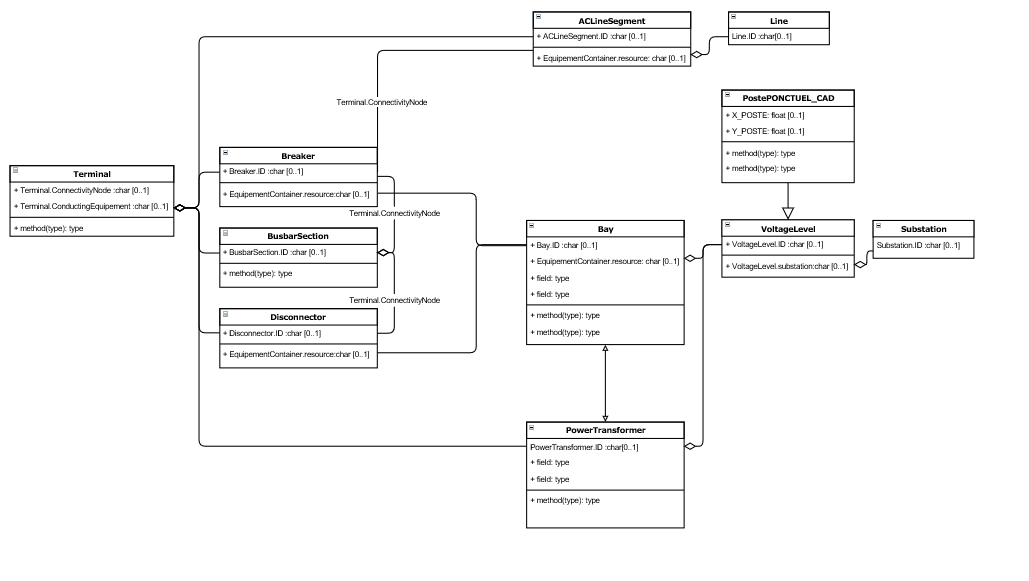
\includegraphics[width=1\textwidth]{0.figuras/Synoptique_UML_classes_RDF_Stanway.png}}
    \captionof{figure}{Classes synoptical dependencies diagram.}
    \label{fig:Classes-synoptical}}
\end{figure}  

On the pursuit of treatment power economizing, just those attributes specifically used for topological structure reconstruction are kept. On top of that, those associated with pictographical properties are evidently kept as well.

Even the lmogic structturing was pretty well formatted and discretional, no support of its UML model was in us. Henceforwarth, its deployment and reconstruction of the Stanway-imported files has been handmade reproduced by cognitive appreciation. 

\subsubsection{Topology reconstruction}
\label{}

Each of these elements classes corresponding to an electric notion (\textit{Breakers, Disconnector, PowerTransformer,} etc.), they are subsequently levelled, then regrouped  and, finally, enriched, as on-field. These dependencies an architecture deployment enabling to parametrize their representation, as shown in \autoref{fig:post_draft}.

\label{subsubsec:AIG:methodology:structurisation:topology}
\begin{itemize}
    \item Henceforth, classes are firstly hierarchically organized in several levels, as in practice, following the criteria shown in the \autoref{tab:classes_XML} below. These levels notion is quite important as it approaches the architecture skeletom to reality's.
\end{itemize}


\begin{table}[h]        \centering
\label{tab:classes_dependences}
\caption{XML classes hierarchical levels and depending attributs}
\begin{tabular}{l|l|l}
\textbf{\textit{Level}} & \textbf{Container} & \textbf{Contained}\\ \midrule
\textit{Lv.4} & Region & SubStation \\ \midrule
\textit{Lv.3} & SubStation & VoltageLevel \\ \midrule
& PowerTransformer & PowerTransformerEnd - Terminal \\
\textit{Lv.2} & ACLineSegment & Line - Terminal \\ 
& VoltageLevel & Bay - BusBarsection \\ \midrule
\textit{Lv.1} & Bay & Disconnector - Breaker - LinearShuntCompensator\\ \midrule
\textit{Lv.0} & Terminal & EquipementContanier - ConnectivityNode\\
\bottomrule
\end{tabular}
\end{table}

\begin{itemize}[label={}]
    \item The hierarchic model present in the XML databases model is built in such a way that every element is kept in relation with those form which it depends along the hierarchic chain, enabling attribute interlying and correspondence easy identification.
\end{itemize}


\begin{itemize}
  \item  Next, once the elements in \autoref{tab:classes_XML} identified, we proceed to the study of their functional dependence and continence relations in connection through \hyperref[fig:post_XML_structure-Terminal]{a coming good representation basis settlement}:
  \end{itemize}
\begin{figure}[h]
    \centering
    \parbox[t]{0.6\textwidth}{
    {\centering
    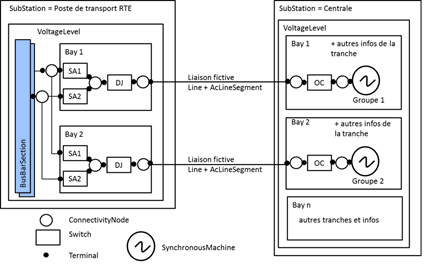
\includegraphics[width=0.6\textwidth]{0.figuras/BusbarSection_dependences_fonctionelles.png}}
    \captionof{figure}{Functional dependencies inside a post, according to XML-hierarchical tree structuring.}
    \label{fig:post_XML_structure}}
\end{figure}



  
    
    \begin{itemize}
        \begin{itemize}
            \item Here is where the \texttt{Terminal} notion appears, extremely important for keeping model connectivity.
       \end{itemize}
    \end{itemize}

\begin{figure}[h]
    \centering
    \parbox[t]{0.6\textwidth}{
    {\centering
    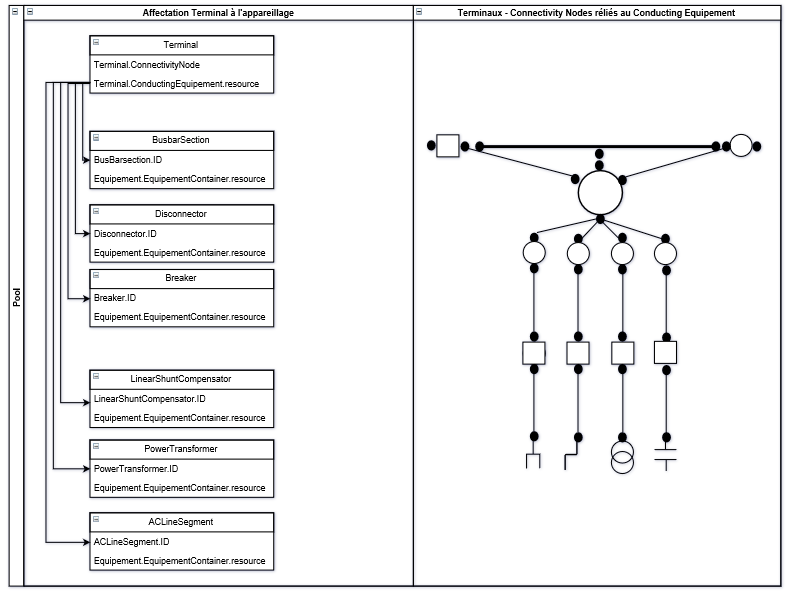
\includegraphics[width=0.6\textwidth]{0.figuras/Connectivite_classes-Notion_Terminal.png}}
    \captionof{figure}{Functional dependencies inside a post, according to XML-hierarchical tree structuring.}
    \label{fig:post_XML_structure-Terminal}}
\end{figure}  

\begin{itemize}[label={}]
        \begin{itemize}[label={}]
\item  As shown in the \autoref{fig:post_XML_structure-Terminal}, elements are not linked directly between them. A terminal let
bus multiple elements interconnection, and, by the way, its introduction clarifies intra-bay dependencies by adding an intermediate stage.
 \end{itemize}
    \end{itemize}
\begin{itemize}[label={}]
        \begin{itemize}
\item \textit{ConnectivityNode} as linker, and \textit{EquipementContainer} as continent let the forming objects to establish 2-way dependencies, as shown in \autoref{fig:Terminal-ConnectivityNode} for the third \textit{BusbarSection} of \texttt{SV.O-P71}, \textit{Saint-Valentin} 400-kV post third bar's (see \autoref{fig:post_draft}).
        \end{itemize}
    \end{itemize}

    \begin{figure}[h]
    \centering
    \parbox[t]{0.6\textwidth}{
    {\centering
    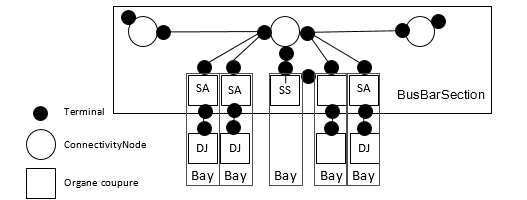
\includegraphics[width=0.6\textwidth]{0.figuras/Terminal_connectivityNode.png}}
    \captionof{figure}{\textit{Terminal} and \textit{ConnectivityNode} notions.}
    \label{fig:Terminal-ConnectivityNode}}
\end{figure}

\begin{itemize}[label={}]
        \begin{itemize}
\item On the basis that a\textit{Bays} and \textit{BusbarSections} are the standard continents of electrical switching devices, thus of \textit{Breakers} and \textit{Disconnectors} in the majority of cases, finally linked between them through \textit{Terminals}. 

\textit{Bays} are destined to represent positions towards other post, and thus their topological structure remains practically unchangable from the \textit{Disconnector-Bay-Disconnector} towards the object off-\textit{VoltageLevel}, whereas \textit{BusBarSections} can be unconcernedly linked by \textit{Breakers} or \textit{Disconnectors}, which will be affected to both terminals of the linking barres in question.

Finally, the topology inter-\textit{BusbarSections} is quite particular, where no notion of continance between the bar switchers and the bar themselves is explicted. 

\end{itemize}


\end{itemize}

  \begin{figure}[ht]
    \centering
    \parbox[t]{0.475\textwidth}{
    {\centering
    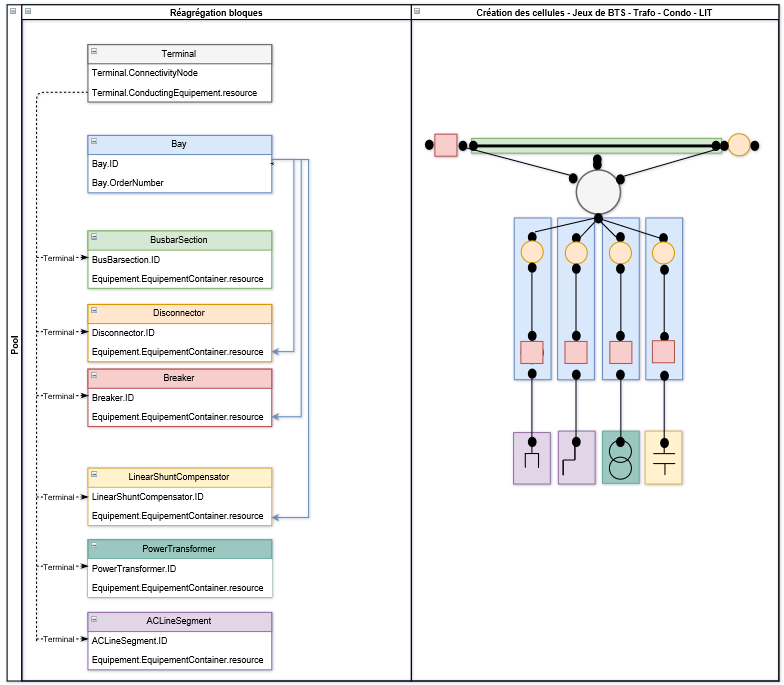
\includegraphics[width=0.475\textwidth]{0.figuras/Cellule_BTS_accroches.png}}
    \captionof{figure}{\textit{Bay} and its containing, plus \textit{BusbarSection} notions.}
    \label{fig:Bay_BusbarSection}
    }
    \hfill
    \parbox[t]{0.475\textwidth}{
    {\centering
    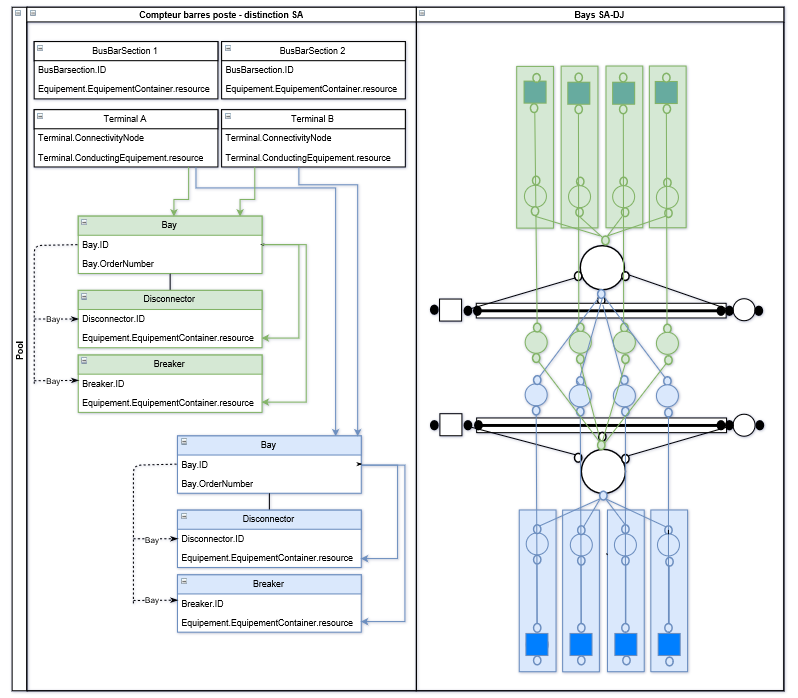
\includegraphics[width=0.475\textwidth]{0.figuras/Union_DJ-SA-Barre.png}}
    \captionof{figure}{\textit{Breakers} are affected to each \textit{Bay - BusbarSection} through \textit{Disconnectors}.}
    \label{fig:Breakers}
    }
\end{figure}

\begin{itemize}[label={}]
        \begin{itemize}
\item To illustrate this example onto group dependencies creation, the same way \textit{Bays} regroup \textit{Disconnector} and \textit{Breakers}, a post (\textit{VoltageLevel}) will contain the abovementioned \textit{Bay} notion, plus \textit{BusBarsection} one. 
\end{itemize}
\end{itemize}


\begin{itemize}[label={}]
        \begin{itemize}[label={}]
 Different \textit{VoltageLevels} are linked, as on field, by \textit{ACLineSegments or PowerTransformers}. Those last been a bit more complex, they include two "terminals" at each of their ends, which are contained in the \textit{VoltageLevel} and are grouped down the class of \textit{PowerTransformerEnd}. 
\end{itemize}
\end{itemize}

\begin{figure}[h]
    \centering
    \parbox[t]{0.475\textwidth}{
    {\centering
    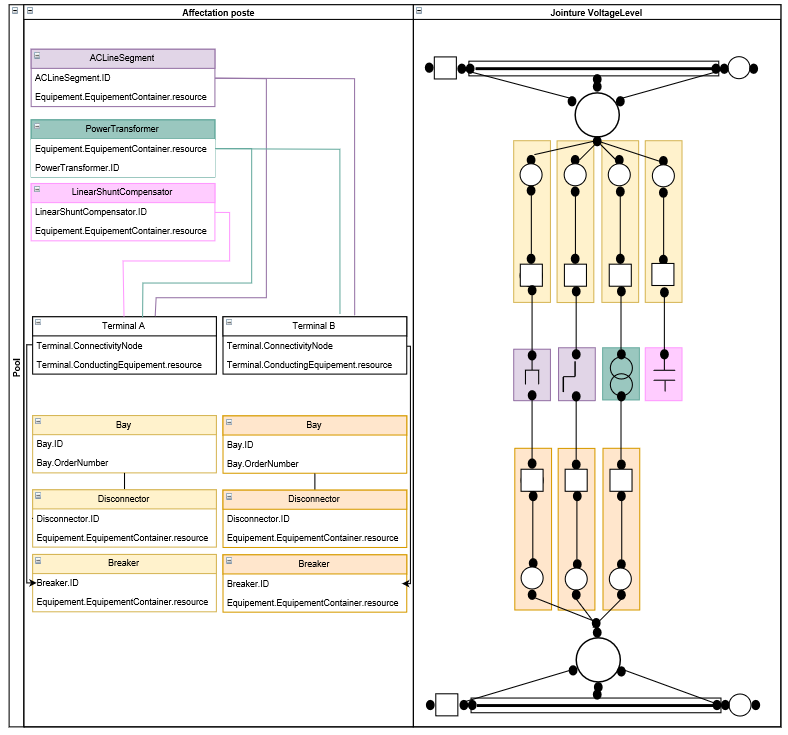
\includegraphics[width=0.475\textwidth]{0.figuras/Jointure_VoltageLevels.png}}
    \captionof{figure}{\textit{ACLineSegment, PowerTransformers} and \textit{LineShuntCompensator} as linking or terminal elements of  \textit{VoltageLevels} respectively.}
    \label{fig:VoltageLevel-interconnections}}
\end{figure}

\begin{itemize}[label={}]
        \begin{itemize}[label={}]
 Analogically, when \textit{BusbarSection} position ends up on a reactive power tool modifier, whether a compensator or a coil, \textit{LinearShuntCompensator} is deployed. 
 
 \nameref{fig:Terminal-ConnectivityNode} takes good note of all these affirmations and schematic representation of the exemplified post seek to easy the model understanding of the reader.
\end{itemize}
    \end{itemize}
    

\begin{itemize}[label={}]
\begin{itemize}

\item Contrarily, a \textit{Disconnector} will be the \textit{EquipementContainer}\footnote{Whose alpha-numeric attribute will be the same as that of the identifier \textit{Disconnector} in question, named \textit{Disconnector.ID}.} of two different \textit{Terminals}, which will be linked to others through the \textit{Terminal.ConnectivityNode} notion.

\end{itemize}
    \end{itemize}

\subsection{Data management}
\label{sub:AIG:data-management}

These classes are interlinked and played with in FME. Two main stages will encompass the natural activity carried out in the software:
\begin{itemize}
    \item Hierarchic chain enrichment through classes merging.
    \item Graphical properties attribution and object displaying configurations.
\end{itemize}

In a second stage, the approach undertaken has seeked to modularize FME treatments, which quite systematical and rigorous, just will require minimal modifications for several specific cases, as that of the \texttt{PowerTransformer-PowerTransformerEnd} linking steps for example. This processus contributing to alligerate considerably the files size, yet as the schematic complexity.

\subsubsection{FME fonctionalities}
\label{subsub:AIG:data-management:FME-fonct}

First of all, attributes are imported in a vast range of different input formats, many of them neatly in Feature-Type XML Reader form, and thereafter a first methodological filtering will be performed, in case several of them re null or found empty.

EXPLICAR LAS DIFERENTES FUNCIONALIDADES DE FME MAS ANADIR SINOPTICO TRATAMIENTO FME

Y QUE ES EL RESULTADO QUE DAN CADA UNA DE ELLAS

\subsubsubsection{\textit{- AttributeFilter}}

In the first placed, not all attributes are always imported from CIM model, on pursuit of performance boosting and discretional workspacing. This is easily feasible thanks to FME Readers, which regardless of the input format enable attribute selecting.

\subsubsubsection{\textit{- FeatureMerger}}

This tool is the most important attribute management operation towards an UML hierarchical para-model creation, which, should be kept in mind, is one of the major contributions of the work undergone towards a solid and robust database patrimony creation. Theoretically speaking, it consists of a mechanism for cross list joining, which related on several \textit{pivotting} arguments.Two list input types enter a \textit{FeatureMerger} on principle: 
\begin{itemize}
    \item \textit{Requestor} will add the main list, that is all the arguments (which will be completely kept unless otherwise specified) remain on the output merged list
    \item \textit{Supplier} will furnish the \textit{Requestor} with as many as \textit{pivotting} arguments stipulated.
\end{itemize}

However, multiple options configuration are available on FME FeatureMerger toolkit, and list are obviously transposable, so are their arguments and pivotal arguments.

\subsubsubsection{\textit{- SubStringExtractor-StringConcatenator}}

Shall be kept in mind that we are continuously working with alpha-numeric chains of characters, which sometimes requires from a thorough, yet symptomatic attribute tailoring. In particular, \textit{pivot} list attributes were systematically prefixed by a #, which shall be taken into account it a consequent pivotal coherence had to be kept among differnet lists. 

\subsubsubsection{\textit{- TestFilter-Sorter}}

Parametric filtering being necessary at times, Test Filtering and List sorting tools resulted to be extremely important to this extent, as coherence could be easily lost otherwise.

For instance, when discerning between breakers positions on top or underneath a post, attribute \textit{Bay.bayOrientation} was studied. Different values of this attributes required different treatments and so that different representation criterias, as shown in \nameref{subsub:AIG:diagram-layout:object-picto-properties} section maxims. It is in this spirit that attribute filtering and sorting may be used for conditions statement and consequent processes divergences introduction.

\subsubsubsection{\textit{- ListBuilder-ListSorter}}

Following the statement up here, elements grouping through list is also extremely important for parametric treatment. Common-sourced elements may be managed equally, and so this feature enables this possibility. On top of that, list can afterwards exploited, there retrieving the same continent structure than before its building.

\subsubsubsection{\textit{- CoordinateExtractor}}

Some elements have intrinsic geometrical properties, which are assigned to them by FME geometrical toolkit creator possibilities such as VertexCreator among others. When extraction of this properties needed, this tool enables its acquaintance for posterior designing or redrafting.

\subsubsubsection{\textit{- VertexCreator}}

The geometric creator by excellence, it enables any 2D geometry (Point, Line, Polygon, etc) creation and has been extensibely used along the treatment because of its simplicity and easy debugging properties.

\subsubsubsection{\textit{- PointConnector}}

Once points created, sometimes is interesting its line-linking according to several properties. This is the case, for example, of \textit{BusbarSection} creation or \textit{Disconnector-Breaker} joining. PointConnector enables all this and other possibilities, providing that elements are well sorted and structured.

\subsubsubsection{\textit{- LineJoiner}}

One step furtuer from PointConnector onto element joining is LineJoiner. That is, once the line created through PointConnector or VertexCreator implementation, they can be likewise linked between them parametrically.

All this toolkit internalized, its deployment can be broadly split on 3 main stages: 
\begin{itemize}
    \item \textbf{Attribute importing and list systematical enrichment}, provoking the whole hierarchical chain slub.
    \item \textbf{Filtering and discernible treatment}, for posterior parametric representation or eventual treatment processes set up.
    \item \textbf{Single-post Diagram layout displaying} according to the metadata nature, with their corespondent \textit{ACLineSegment} linking inter-post lines.
\end{itemize}

That is, through list merging, attributes are incorporated to their UML model, showing functional dependencies between classes off.

When necessary, certain exceptional treatment are implemented, always keeping a systematical rigorous approach. 

Depending on nature and parametric properties, different displaying are performed, by different pictographcial properties affectation

Whole process can be found on \nameref{Acronyms} chapter. NANDIR TODO EL ESQUEMA UNA VZ TERMINADO ( AQUI SOLO MOSTRARLO POR PARTES)

EXPLICAR PROCEDIMIENTO PASO A PASO INTRODUCIENDO A CADA VEZ LOS ESQUEMAS PARCIALES DE CONEXION DE CLASES - ATRIBUTOS??

GRAN ESQUEMA DE CONEXION DE LAS CLASES CON ARGUMENTOS CLAVE Y PROCEDIMIENTO PASO A PASO

\subsection{Diagram layout drawing}
\label{sub:AIG:diagram-layout}
Once the different classes levelled and their bounding hierarchical links identified, the time to attribute functional dependencies and implement their diagram layout, in a first stage in a post separated format followed by an integrating procedure, plus a space-optimization seeking. As the step between \autoref{fig:CIM_diagram-layout-skeleton} and \autoref{fig:CIM_diagram-layout} shows, every class notion correspond to an electric element, whose representation form is standardized and spread following \autoref{subsub:AIG:normative:elec-representation} specifications, which will be deeply tackled in detail in the following section \ref{subsub:AIG:diagram-layout:non-eq-notion}. 

All those elements will not be unconditionally represented on the pursuit of cache memory optimization\footnote{And specially taking into account that Herge's team-lead is finally seeking to exploit its layout in a tablet format, which will compromise even more strongly display featuring.}, but may remain in the skeleton architecture reproduction. In this way, we will perform a conditional displaying as we zoom out or in throughout the SRC and SNC schemes under the condition that no more than 10 000 objects per screen will ever be represented, with a seeked optimal number of about 8 000. 

\subsubsection{Non-equivoque notion}
\label{subsub:AIG:diagram-layout:non-eq-notion}

It is certainly important when transposing the structure to the drawing to rigorously represent every element for a non-equivoque layout of the on-field electrical structuring. In other words, each element unity shall remain unchanged all the treatment long, regardless of the enrichment process it may undergone. 

For separate unit components representation and posterior assembling, it is primordial to keep these notions unaltered in seek of a two-sided bijectional relation between databases and diagram layout representation.

Additionally, all these model solidity maxims could be implemented through \textit{DupplicateFilter} FME toolbox functionality. called , which keeps just one unique element per identifier.

NAME SUBSPACES AND PHOTO OF BIJECTIONAL SPACES RELATION THEN USE SAME NOTATION FOR APPARTAT HEREAFTER

\subsubsection{Object unalterepictographic properties attribution}

\label{subsub:AIG:diagram-layout:object-picto- properties}

Position plus, altogether with the pictographic icon, discussed in \nameref{sec:approach:software:ArcGIS} section aofterwards, will be the two main properties to assign to an element. Therefore, position will be created by the operation of two coordinated systems: the local one of the intrapost himself \(\lbrack \mathscr{X}_{local}, \mathscr{Y}_{local}  \rbrack \), and that of the macro post position inside the whole representation scheme, e.g. \(\lbrack \mathscr{X}_{origen puesto},{Y}_{origen puesto} \rbrack \), who will be the one to optimize on \nameref{subsub:AIG:SLV:graph_theory} subsection.

Devices will be systematically positioned in accordance to, in first, the fonctional dependencies with another objets, plus their given attributes as \textit{Classes} (\texttt{Bay.Bayorientation}, and \textit{SCADA step} neatly, as shown \hyperref[fig:post_draft]{hereafter}).

\begin{figure}[h]
    \centering
    \parbox[t]{1\textwidth}{
    {\centering
    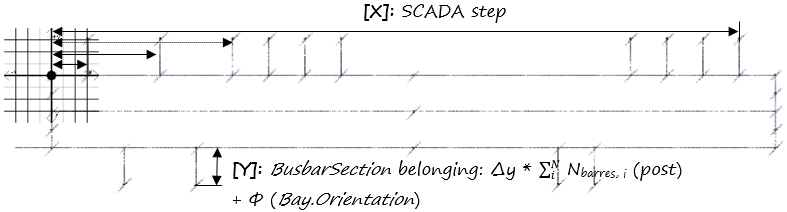
\includegraphics[width=1\textwidth]{0.figuras/Draft-post-represenation.png}}
    \captionof{figure}{\textit{Saint-Valentin} (\texttt{SSV.O-P71}) post first FME representation draft, with its local coordinates position parametric model.}
    \label{fig:post_draft}}
\end{figure}

Thus, the subspace general coordinates \(\lbrack \mathfrak{X}_{general}, \mathfrak{Y}_{general} \rbrack \) of a certain element, contained within a post, will be expressed as the linear combination\footnote{for easying elements magnitude in contrast with post gapping.} of \(\lbrack \mathscr{X}_{origen puesto},{Y}_{origen puesto} \rbrack \) and \(\lbrack \mathscr{X}_{local}, \mathscr{Y}_{local}  \rbrack \) subspaces:
\\


\begin{equation}  \left\lbrace
\begin{array}{cc}
     & {\mathfrak{X}_{general}}=\mathscr{X}_{Post origin}+\mathscr{X}_{local}  \\
     & {\mathfrak{Y}_{general}}=\mathscr{Y}_{Post origin}+\mathscr{Y}_{local}
     \end{array}
     \right.
    \end{equation} 

Being the post coordinates fixed as in the following, they will be matter of long study in \autoref{subsub:AIG:SLV:graph_theory}:
ling Breaker's 

\begin{itemize}
    \item \(\mathscr{X}_{local}=0 \leftrightarrow\mathfrak {X}_{general}=\mathscr{X}_{Post origin}, \) placed on the left-sided Coupling Breaker's x-axis. 
    \item \(\mathscr{Y}_{local}=0 \leftrightarrow\mathfrak {Y}_{general}= \mathscr{Y}_{Post origin}, \) placed on the first BusbarSection's y-axis.

\end{itemize}
From the post introspective PoV, objects local positioning \(\lbrack \mathscr{X}_{local}, \mathscr{Y}_{local}  \rbrack \)  must be systematically parametrized in a rigorous way so that every element positioning is completely unique and faithful, his fundamentals raising no doubts about which criteria was approached for it. 

In this purpose, and once post position local origin establishedon the first bar at the coupling elements-high, as shown in \autoref{fig:post_draft}, objects coordinates will be referred to this origin. To this effect, the main variables which will be used to parametrize those positions in the following are:

\begin{itemize}[label={-}]
\item \texttt{Bay.bayOrientation}
\item \textit{SCADA step} \footnote{In DPC\textsuperscript{2} files, \textit{Pas} \quad \textit{SCADA} is given in multiples of 10\cite{cahier_dpc2}.}
\end{itemize}
 
Being the position breakers the firsts to be placed, every post elment position will be 2Dimensionally-referenced to this following these rules:

\subsubsubsection{- Breakers}
\begin{equation}
\mathscr{X}_{local}= \frac{SCADA & step}{10}    
\end{equation}

For example, \autoref{fig:post_draft} shows \textit{Saint-Valentin} post behaviour in \textit{Lille}-SRC zone, the \texttt{Bay.bayOrderNumber} argument fixes the horizontal position\footnote{Being the first coupling (if existing) situated on the zero of abscisa axis}, while the \texttt{Bay.orientation}, plus the adherence to a certain bar out of the total number in the post will determine its vertical's:


\( \mathscr{Y}_{local}=231321\) will be generatlly formulled as \( amfjaf\), which finally will declinate, in fonction if \textit{Bay.bayOrientation} vaule is \(\mathsf{H}\) (up) or \(\mathsf{B}\) (down) onto:

\begin{equation}  
\mathscr{Y}_{local}=\left\lbrace
\begin{array}{llllll}
     & \textit{Bay.bayOrientation} & =\(\mathsf{H}\) &\Longrightarrow &\mathscr{Y}_{local}^{up}=1 \\
     &  \textit{Bay.bayOrientation} & =\(\mathsf{B}\) &\Longrightarrow & \mathscr{Y}_{local}^{down}=\sum_{n=1}^{\ N_{bars}^{max}} (1-n) * \Delta y^{SA}  & \forall n \in \mathbb{N}
     \end{array}
     \right.
    \end{equation} 

\subsubsubsection{- Coupling breakers}

Coupling breakers are normally place at the beginning or in the end of the bar, which is already taken into account in their \textit{SCADA step} parametric initialization. Anyway, this last will be subsequently verified for every of these elements in line with the following equations:
\\
\begin{equation}
    \mathscr{X}_{coupl. breaker}=\left\lbrace
\begin{array}{llllllll}
     & \textit{Bay.bayOrderNumber} & =\(\mathsf{0 - Left}\) &\Longrightarrow &\mathscr{X}_{coupl. breaker}^{left}=0 \\
     & \textit{Bay.bayOrderNumber} & \neq\(\mathsf{0 - Right\footnote{max_i(X_positions(poste i))}}\) &\Longrightarrow &\mathscr{X}_{coupl. breaker}^{right}=max (\mathscr{X}_{positions}) & \forall n \in \mathbb{N}
     \end{array}
     \right.
\end{equation}

\subsubsubsection{- Bars}

Bars are drawn as lines by aggregating in X the different positions linked to the correpsondent \texttt{BusbarSection}-linked ouptut positions, whereas Y position will depend on a counter of \texttt{BusbarSections} belonging to the \texttt{VoltageLevel} in question.

For the abscis coordinate, they are thereafter drawn in fonction of the maximum and minium (\( \mathscr{X}_{local}^{max}\) to \( \mathscr{X}_{local}^{min}\)) positions of the bar to whom the devices belong.

\begin{equation}
    aa
\end{equation}


Decoupage barre en BTS
Positionnement celllules BTS
Elementos diferentes e independientes



\subsection{Problems faced}

Several unexpectted problems have been encountered as project advanced, being all of them presented herafter. In addition, the wy they were identified, tackled then solved is exhaustively explained, being the \textit{modus operandi} itself more interesting thatn the final output of it ijn most cases.

The methodology followed to achieve the objectives is shown in Figure
1.3. As can be seen, this work consist of ve main tasks, organized in several
chapters.
Chapter 2 deals with the literature survey of current strategies to optimize
engine efficiency. In this sense, a comprehensive review is performed
to understand the engine research background over the last 2 decades. The
trade-o between emissions and eciency, along with the potential of thermal
balance for engine evaluation is discussed in this chapter. An extensive amount
of works dealing with RICE thermal balances is used for the discussion, where
the importance of establishing a comprehensive methodology for its analysis
is evidenced.
Chapter 3 shows a complete description of the experimental installations
and the reference thermodynamic model, including:
 Details of the instrumentation required to perform the experimental
work.
 A description of the dierent sub-models included in CALMEC and SiCiclo
(0D thermodynamic tools), detailing which of them need to be further
upgraded as done in the following sections.
Based on the experimental and modelled information available, Chap-
ter 4 introduces an integral experimental and modelling methodology to perform
the thermal balance, called Global Energy Balance (GEB). This methodology
considers 2 main points of view, on the one hand the External GEB,
which considers the engine as a black box and whose terms are obtained mainly
through experimental techniques; and on the other hand the Internal GEB,
which takes into account all the internal energy degradation phenomena due
to thermal and mechanical processes (e.g. heat rejection and friction). For the
sake of completeness, the relationship between internal, and internal-external
terms will be also detailed in this chapter. Special analysis of some heat rejection
terms used for the calibration and validation stages will be provided,
along with an experimental uncertainty analysis.
Taking into account the description of the energy terms provided in
Chapter 4, the improvement of some reference sub-models and the proposal 
of new ones will be necessary. Therefore, Chapter 5 is dedicated to the
development and validation of specic heat transfer and mechanical losses
sub-models, along with a comprehensive uncertainties adjustment process.
To asses the potential of the methodology developed in this work, Chap-
ter 6 describes the use of the GEB in two dierent engines: one conventional
1.4 Methodology 9
multi-cylinder 4-stroke Diesel engine, and a research single-cylinder engine.
The work presented in this section is divided in 2 steps:
1. Description of the sub-models calibration methodology based on the
equivalent heat transfer terms presented in Chapter 4, along with the
uncertainties tuning described in Chapter 5.
2. Performing the GEB analysis in some parametric variations, aimed at
the integral energy characterization of the studied engines, along with an
example of the use of the calibrated sub-models and GEB for predictive
applications (using a 0D thermodynamic model).
Finally, Chapter 7 summarises the work performed and shows the main
conclusions regarding its contributions. In addition, some proposals for future
works are lastly discussed.
For convenience, besides each chapter bibliography, at the end of this
document all the references cited are organized in alphabetic order, indicating
the pages where they are cited.

ANADIR QUIZA UNA TABLA DICIENDO LOS DIFERENTES PROBLEMAS IDENTFICAIDOS + COMO HAN ISDO ABORDADOS A NIVEL TECNICO( AUE DIFICULTADES ADICIONALES PODRIAN DECRIVARSE DE EZTO) Y CUAL HA SIDO LA SOLUCION FINAL IMPLEMENTADA

Several problems have been encountered when layout diagram representation
\subsubsection{LITs crossing}

Due to the massive amount of post to represent, apart from  the objective divergence between concomitant projects in the matter, we finally were encountered with a multiple \textit{ACLineSegment} crossings, being the post origin position the root of the problem

Three-linked at a time post were triangulated, its circle identified and set in common for the three of the them

ANADIR FOTO ANTES DESPUES

\subsection{Technical issues}
\label{subsub:AIG:technical-issues}

Constituting the graphical interface for the most part of Rte's on-field business users, an important flux of financial actives depend on Herge's fate, which makes it a substantially constrained project in terms of users necessities. They are the ones who grab the major part of the negotiating power and therefore encompassing the trail of the project.

Consequently, the results of the displayed methodology shall remain certainly close to the actuals, and changes may be considerably evident, flexible and easily apprehensible. This incertitude reigning all the project long has deeply impacted its approach and methodology, always on the pursuit of flexibility by means of modularity and adaptability possibilities in connection to the future additional steps Herge could take, yet as all its impacted partners.

In keeping with the aforementioned maxim, an additional difficulty pop up: notably, several technical issues have been accordingly identified throughout the complete project, whom could be systematically approached and dealt with, a well-focus approach beforehand has disminuiss their imapct and let to identify most of them in advance.

In this concept, FME treatments have been performed the most modularized possible, through the use of versionable \textit{Customer Transofmers}, which could be update to each upgrading or modification of the treatment "alpha". Once its use exhausted, ArcGIS tools were maximally developed and in the most logical way, using the \textit{Network Analyst} toolpackage first and foremost, as it was the one that most approached our technical needs.

Specifically, two main difficulties encompassed the unexpected problematics abborded: 

\begin{itemize}
    \item First of all, crossing-lines between post problems were appreciated, specially when charging big areas of study\footnote{Which seems completely normal, taking into account the electrical network is finally a growing mesh, for ensuring a good clients level of service, plus flexibility in maintenance and exploitation.} 
    \item The second problematic refers to several problems occurred regarding post problems management at each iterative step on ArcGIS, which compelled to objects overlapping fixing, ended sometimes on recurrent overlapping. This was due to a non-adequate post position changes awareness, blocking graphs algorithm from taking into account the new situation of the modified post-positions-matrix.  
    \end{itemize}

Anyway, these problems have been correctly addressed and finally solved, as shown in \hyperref[susub:AIG:technical-issues:postpositionmanagement]{the following subsection}, for attaining functional \nameref{sub:AIG:technical-issues:proposed-solutions}. Altogether with a good technical documentation of the chosen decisions, the extra effort linked to the previously stated will enable to lighten future actions during the subsequent versions of Herge.

\subsubsection{Recurrent post position management acknowledgement}
\label{subsub:AIG:technical-issues:postpositionmanagmement}

As previously stated, if we are seeking to automatize the post position in a recurrent basis, there must be a way of acknowledging which approach have been performed plus reloop those position in the canonical algorithms. 

\subsection{Proposed solutions}
\label{sub:AIG:technical-issues:proposed-solutions}

 Envisablable solutions have been strivedfrom an ArcGis basis, on which \textit{Network Analysis} tools enabled automatic management of post position, building on a Graph theory theoretical background.
 
\section{Layout optimization}
\label{sec:AIG:layout_optimization}

The last stage of the work undertaken was to be able to manage post position so that the whole layout may be optimized. A double slope opens  both theoretically and practically.

This way, from one hand a theoretical background documentation has been proceeded of a correct industrialized state of art conscience raising. 

\subsection{Principe}

The intersection of different methodological techniques have enabled the open up of a logical implementation of post position optimization.

\subsection{Theoretical background}
\label{sub:AIG:SLV:theoretical background}

As underlied in the section \ref{sub:AIG:normative}, no industrialized documentation and complete lack of framework has been stated on most of the techniques implemented through this work. Their avnant-garde statusli and strictly research-scope character prevents its technical transportation from already undertaken on corporate projects. There lays also the interest of this study ,as recurrently ennounced.

\subsubsection{Graph theory}
\label{subsub:AIG:SLV:graph_theory}

Well-spread on the treatment of geodatabase information exchange, graph theory has been extensively developed in the end of 80s, and 90s. This process us consisting on relative weight assignation of different resources, lets correlative solution layout optimization, its exploitation o n electrical diagrams optimization remains notably unexploited.

Force-based network representation as that of \hyperref[fig:force-diagram]{the following diagram}

\begin{figure}[h]
    \centering
    \parbox[t]{1\textwidth}{
    {\centering
    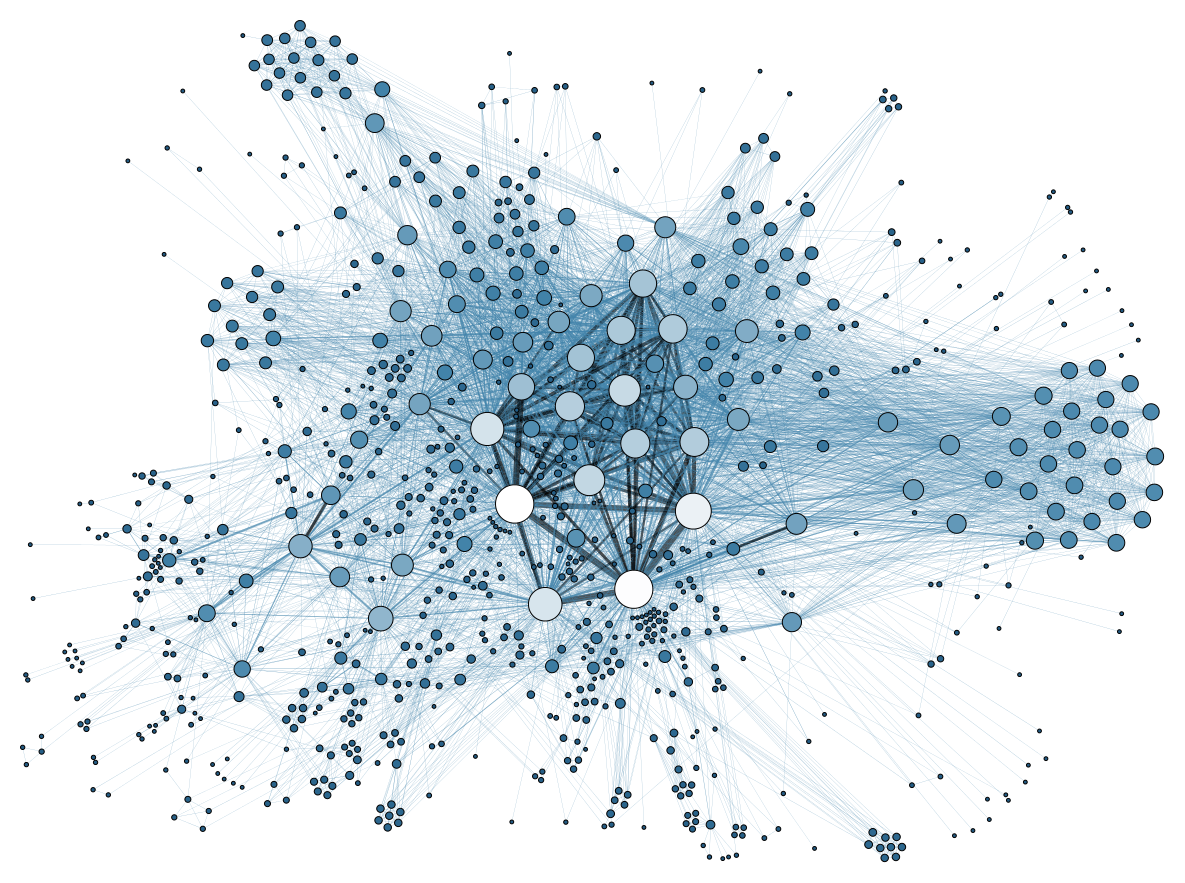
\includegraphics[width=1\textwidth]{0.figuras/Social_Network_Analysis_Visualization.png}}
    \captionof{figure}{Force diagram assessment performed on a social network analyst visualization.(\href{https://en.wikipedia.org/wiki/Graph_drawing}{Wikipedia-sourced})} 
    \label{fig:force-diagram}}
\end{figure}

\subsubsection{Metaheuristic algorithms}
\label{subsub:AIG:SLV:graph_theory:meta_algorithms}

On the pursuit of automatizing data dumping, yet as characterisitical cases treatment, several methaheuristic algorithms have been systematically introduced. Their functioning basis remain on the principle of anomalies creation, plus their propagation thought the hierarchical chain, serving to create unthinkable situations. Those anomalies will not get reproduced anymore as it happens, for instance, in the evolution chain theory of Lamarck, the one on whom the Metaheuristic algorithms relay.

\subsubsection{Voronoi diagrams}
\label{subsub:AIG:SLV:Voronoi}

In mathematics, a Voronoi diagram is a partitioning of a plane into regions based on distance to points beforehand specified in a certain subset of the plane. Through Delaunay triangulation of a set of points is dual to its . 

\begin{figure}[h]
    \centering
    \parbox[t]{0.7\textwidth}{
    {\centering
    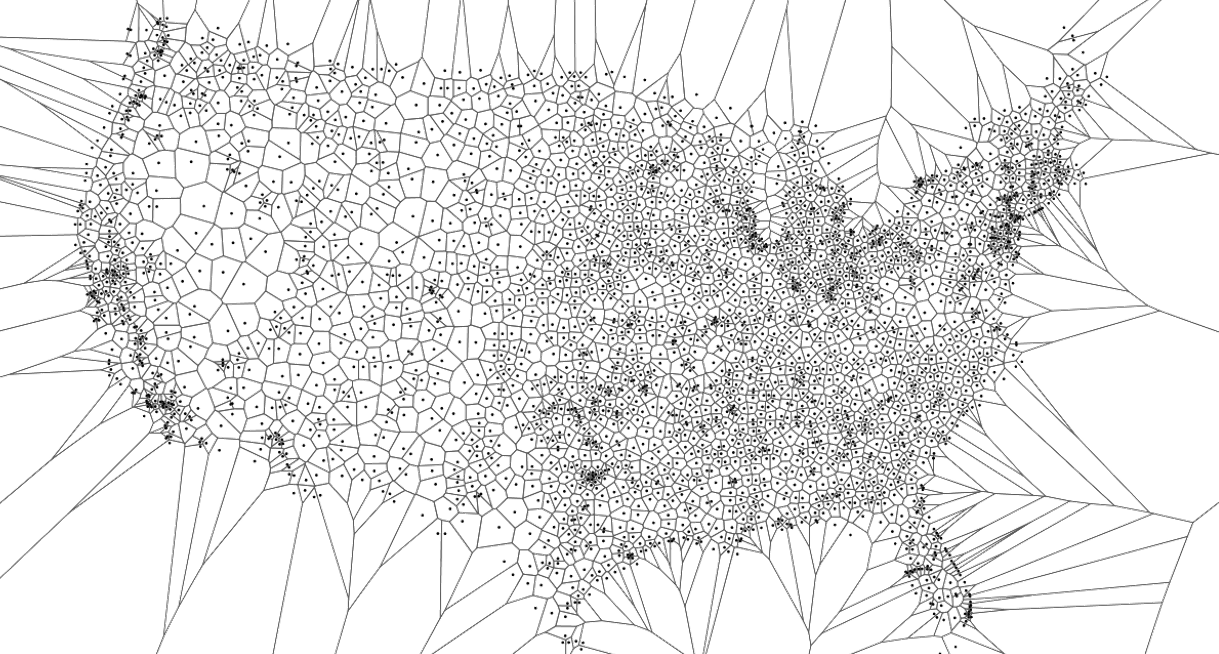
\includegraphics[width=0.7\textwidth]{0.figuras/Usa_airports_voronoi_diagrams.png}}
    \captionof{figure}{Force diagram assessment performed on a social network analyst visualization.(\href{https://en.wikipedia.org/wiki/Voronoi_diagram}{Wikipedia-sourced})} 
    \label{fig:Voronoi-diagram}}
\end{figure}

To our case of study, they let to characterize the relational dependencies implementation of relational databases. And what is more important, its application was already integrated in FME toolkit, what lighten notably up its implementation and supposed no derives regarding the previous approach.

In geometry, Voronoi diagrams can be used to find the largest empty circle amid a set of points, and in an enclosing polygon; e.g. to build a new supermarket as far as possible from all the existing ones, lying in a certain city.
Voronoi diagrams together with farthest-point Voronoi diagrams are used for efficient algorithms to compute the roundness of a set of points. The Voronoi approach is also put to good use in the evaluation of circularity/roundness while assessing the dataset from a coordinate-measuring machine.
Modern computational geometry has provided efficient algorithms for constructing Voronoi diagrams, and has allowed them to be used in mesh generation, point location, cluster analysis, machining plans and many other computational tasks.


\subsubsection{MDS}
\label{subsub:AIG:SLV:MDS}

Multidimensional scaling (MDS) 

\subsection{Practical solutions}

Once enough theoretically formed, their implemetnation on the \nameref{sec:approach:software} deployment has supposed several challenges, and therefore introduced new milestones in a development approach.

\subsubsection{Maching learning}
\label{sub:AIG:machine_learning}

Well-spread in the latter years, machine learning enables data scientists to systematically acknowledge intelligently classified situations, and therefore perform systematical algorithms in concordance.

\subsubsection{ArcGIS optimization tools}

GIS tools are deeply exploited in cartography and geographical decisions taking assessment processes. 

Regarding our case of study, its toolkit, and notably \textit{Network Analyst} functionality enabled the different post position acknowledgement, plus their management in order to a more intelligent space optimization.

\subsubsubsection{Network Analyst}

This ArcGIS extension functionalities range are apparently inexhaustive regarding geodatabase intelligent management processes, e.g behaviour predicting, meshes of any nature analyzing, among others.

Traditional questions in geographical optimization such as shortest-path finding, business optimal geoexpansion, 5-minutes zone regrouping or the notably famous paradigm of the\textit{Seven Bridges of Königsberg} are easily answered on GIS software. 

Network Analyst fundamental algorithms help assessing this kind of questions and others. Regarding the subject ofour study, a certain network mesh, formed by different post positions, plus the linking lines among them, was presented. The aim was to subsequently optimize these positions in seek of minimizing LITs length and crossing with others. 

This algorithms seemed to respond quite accurately to the presented needs, additionally contributing with unknown fucntionalities that certainly enriched the whole intelligent procedure.
% -------------------------------------



	


% ---------------------------------------------------------------------
% ---------------------------------------------------------------------
% ---------------------------------------------------------------------
% Fin
